In this chapter, we are going to present the background information that is necessary for our approach.
What are neural networks?
How can we test them, and what is spectrum-based fault localization?
\section{Neural Networks}\label{sec:neural-networks}
Without further ado, we will discuss what neural networks are and how they are composed.
We describe what a layer is and what types there are.
For what do we need optimizers and activation functions and what types are there.
Neural Networks are useful in a multitude of fields like classification, regression, transcription or machine translation \cite{goodfellow_deep_2016}.
Neuronal networks are composed of layers, which are composed of neurons.
The neuron is the computational component in a deep neural network.\\
A neuron transforms a vector of inputs $\mathbf{x}$ to the output $y$, $\mathbb{R}^n \to \mathbb{R}$
by using a vector of weights $\mathbf{w}$, a bias $b$ and an activation function $f$ as seen in equation \ref{eq: NeuralFunction}.
\begin{equation}
    y = f\left( \sum^n_{i=1} w_i\cdot x_i + b\right)
    \label{eq: NeuralFunction}
\end{equation}
For example the machine learning software library TensorFlow, which is based on Keras, uses by default Glorot uniform initializer \cite{noauthor_tfkeraslayersdense_2023,glorot_understanding_2010}, for the weights and initializes the bias with zeros.\\
Another important component, are the activation functions, one of the most common ones is the sigmoid function, which is today mostly used in output layers.
The rectified linear unit, short ReLU \cite{fukushima_cognitron_1975,glorot_deep_2011}, as seen in Function \ref{eq: relu}, enables a better training for a neural network compared to the formerly common sigmoid function.
\begin{equation}
    f(x) =
    \begin{cases}
        x& x > 0\\
        0& x <= 0
    \end{cases}
    \label{eq: relu}
\end{equation}
Another, even more promising activation function is the Gaussian Error Linear Unit, short GELU, seen in function \ref{eq: relu}, which was proposed by Hendrycks and Gimpel in 2016 \cite{hendrycks_gaussian_2016} is used by natural language processing models like BERT \cite{devlin_bert_2019}.
It does not just set all negative values to zero like ReLU but weights them.
The differences can be seen in the figure. \ref{fig: activation function}
\begin{equation}
    f(x) = 0.5x\left ( 1+\tanh\left [ \sqrt{\frac{2}{\pi}}\left ( x+0.044715x^3 \right ) \right ] \right )
    \label{eq: gelu}
\end{equation}
\begin{figure}
    \centering
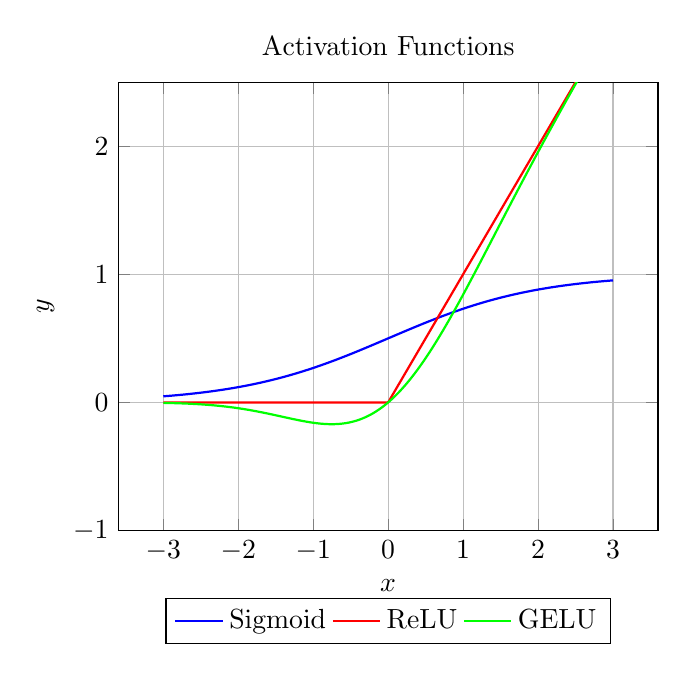
\begin{tikzpicture}
    \begin{axis}[
        title={Activation Functions},
        xlabel={$x$},
        ylabel={$y$},
        domain=-3:3, % Adjust the domain for a narrower x-axis range
        ymin=-1, % Set y-minimum
        ymax=2.5, % Set y-maximum
        samples=400, % Increase the number of samples for a smoother curve
        grid=both,
        legend style={at={(0.5,-0.15)}, anchor=north,legend columns=3},
      ]
      \addplot[blue, thick] {1/(1 + exp(-x))};
      \addplot[red, thick] {max(0, x)};
      \addplot[green, thick] {0.5*x*(1 + tanh(sqrt(2/pi)*(x + 0.044715*x^3)))};
      \legend{Sigmoid, ReLU, GELU}
    \end{axis}
  \end{tikzpicture}
  \caption{Activation Functions}
  \label{fig: activation function}
\end{figure}
The neurons are then combined into layers, in a Deep Neural Network (DNN) we have three types of Layers:
Input layers, output layers and the hidden layers.
There is one input and one output layer, but there is a plurality of hidden layers, as you can see in the figure \ref{fig: neural network}.
The input layer, processes the input for the hidden layers, for example, it converts a 2-dimensional picture to a 1-dimensional array, which can then be processed by the subsequent hidden layers.
The hidden layer performs most of the computational work of a DNN, it works based on the neural equation, that can be seen in the function \ref{eq: NeuralFunction}.
The output layer takes the output of the last hidden layer and transforms it to produce a meaningful output.
In the case of regression or binary classification, there is usually only one neuron, but for multi-class classification, the amount of neurons corresponds to the amount classes to be classified.
The output layer follows the same principle as the formula above, but it does not use a ``normal'' activation function.
Either a linear activation function or no activation function is used for regression, or the softmax function, which can be seen in the function \ref{eq: softmax}, is used for classification models.
\begin{equation}
    f(x_i) = \frac{e^{x_i}}{\sum^n_{j=1}e^{x_j}}
    \label{eq: softmax}
\end{equation}
\begin{figure}
  \centering
  % Input layer neurons'number
  \newcommand{\inputnum}{5}

  % Hidden layer neurons'number
  \newcommand{\hiddennuma}{6}
  \newcommand{\hiddennumb}{8}
  \newcommand{\hiddennumc}{5}

  % Output layer neurons'number
  \newcommand{\outputnum}{4}

  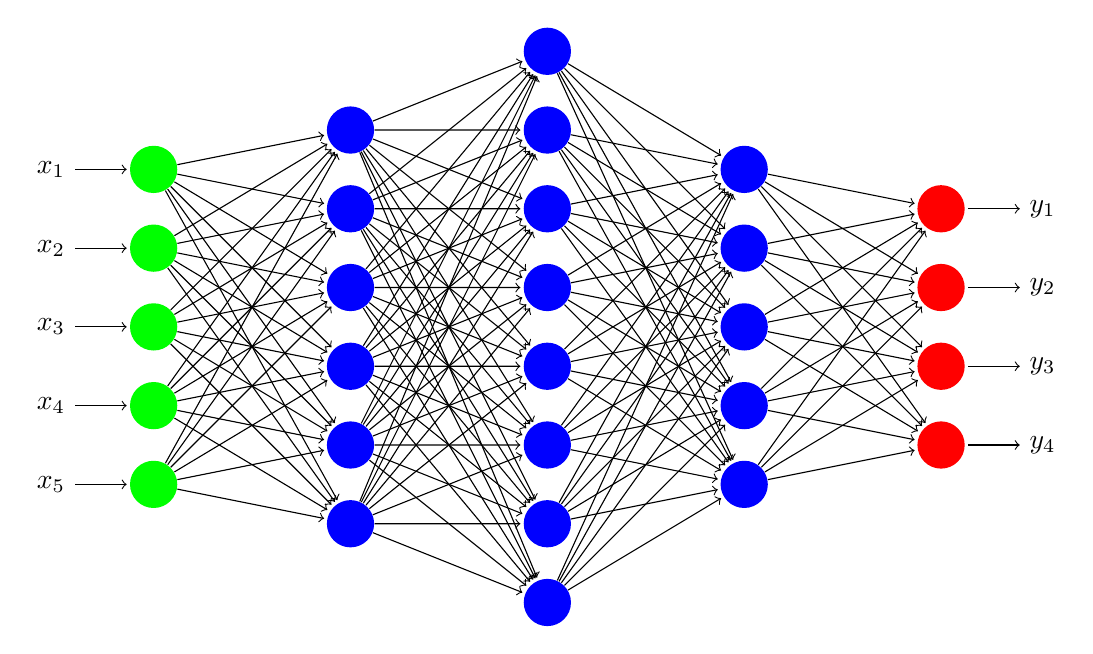
\begin{tikzpicture}

    % Input Layer
    \foreach \i in {1,...,\inputnum}
    {
	  \node[circle,
		minimum size = 6mm,
		fill=green] (Input-\i) at (0,-\i) {};
    }

    % Hidden Layer
    \foreach \i in {1,...,\hiddennuma}
    {
      \node[circle,
		minimum size = 6mm,
		fill=blue,
		yshift=(\hiddennuma-\inputnum)*5 mm
	  ] (HiddenA-\i) at (2.5,-\i) {};
    }

    \foreach \i in {1,...,\hiddennumb}
    {
	  \node[circle,
		minimum size = 6mm,
		fill=blue,
		yshift=(\hiddennumb-\inputnum)*5 mm
	  ] (HiddenB-\i) at (5,-\i) {};
    }

    \foreach \i in {1,...,\hiddennumc}
    {
	  \node[circle,
		minimum size = 6mm,
		fill=blue,
		yshift=(\hiddennumc-\inputnum)*5 mm
	  ] (HiddenC-\i) at (7.5,-\i) {};
    }

    % Output Layer
    \foreach \i in {1,...,\outputnum}
    {
	  \node[circle,
		minimum size = 6mm,
		fill=red,
		yshift=(\outputnum-\inputnum)*5 mm
	  ] (Output-\i) at (10,-\i) {};
    }

    % Connect neurons In-Hidden
    \foreach \i in {1,...,\inputnum}
    {
	  \foreach \j in {1,...,\hiddennuma}
	  {
		\draw[->, shorten >=1pt] (Input-\i) -- (HiddenA-\j);
	  }
    }

    % Connect neurons Hidden
    \foreach \i in {1,...,\hiddennuma}
    {
	  \foreach \j in {1,...,\hiddennumb}
	    {
		  \draw[->, shorten >=1pt] (HiddenA-\i) -- (HiddenB-\j);
	  }
    }

    \foreach \i in {1,...,\hiddennumb}
    {
	  \foreach \j in {1,...,\hiddennumc}
	    {
		  \draw[->, shorten >=1pt] (HiddenB-\i) -- (HiddenC-\j);
	  }
    }

    % Connect neurons Hidden-Out
    \foreach \i in {1,...,\hiddennumc}
    {
	  \foreach \j in {1,...,\outputnum}
	    {
		\draw[->, shorten >=1pt] (HiddenC-\i) -- (Output-\j);
	}
  }

  % Inputs
  \foreach \i in {1,...,\inputnum}
    {
	  \draw[<-, shorten <=1pt] (Input-\i) -- ++(-1,0)
		node[left]{$x_{\i}$};
    }

  % Outputs
  \foreach \i in {1,...,\outputnum}
    {
	  \draw[->, shorten <=1pt] (Output-\i) -- ++(1,0)
		node[right]{$y_{\i}$};
    }

  \end{tikzpicture}
  \caption{Neural Network}
  \label{fig: neural network}
  \fcolorbox{black}{green}{\rule{0pt}{6pt}\rule{6pt}{0pt}}\quad Input Layer \quad
  \fcolorbox{black}{blue}{\rule{0pt}{6pt}\rule{6pt}{0pt}}\quad Hidden Layer \quad
  \fcolorbox{black}{red}{\rule{0pt}{6pt}\rule{6pt}{0pt}}\quad Output Layer
\end{figure}
But, how are deep neural networks trained? \cite{lecun_deep_2015}
The first step is forward propagation, the training data is fed in to the network and flows through the layers, where each neuron performs it operation, according to the function \ref{eq: NeuralFunction}.
Afterward the backpropagation or backpropagation of error is performed. \cite{rumelhart_learning_1986}
Then the output is compared to the desired outcome of the training data, hence, if the predicted outcome of the network matches the actual outcome.
If it doesn't match, it calculates how far off the prediction is.
The process of backpropagation is initiated, which uses an algorithm like Stochastic Gradient Descent (SGD) or one of its modern successors like Adam.
SGD is an iterative method used to optimize an objective function, making it particularly advantageous for high-dimensional optimization problems.
With each iteration SGD updates the model parameters by using the gradient of the loss function concerning the parameter.
This isn't done for the whole dataset but just some data points.
The learning rate describes how far a parameter is changed in the direction of a derivation for one iteration, in SGD this Learning Rate is constant and manually set.

Adaptive Moment Estimation (Adam) \cite{kingma_adam_2017} is one of the successors of SGD. Adam, uses a variable learning rate, which is adapted for each parameter, which uses the estimation of the first moment, the mean, and the second moment, the variance to change the learning rate.
Then this process is repeated until we are gone through the entire training set, which is called an epoch.

\subsection*{Core Layers in Neural Networks}\label{subsec:core-layers-in-neural-networks}
In the following, we will discuss the core layers in neural networks, which are the dense layer, the convolutional layer and the pooling layer.
We use them in our evaluation, hence, we will discuss them in detail.
\subsubsection{Dense Layers}
It is characterized by its fully connected architecture, like seen in the figure \ref{fig: neural network}, meaning every node of the layer is connected to every node of the predecessor layer and every node of the successor layer.
Dense layers are pivotal in learning intricate patterns from data, their versatility allows them to be stacked where each layer captures different levels of data abstraction.
The theoretical function of a dense layer can be seen in the function \ref{eq: DenseLayer}.
Where $x = (x_1,x_2,\dots,x_n)^T$ is the input vector,
$W = \left(\begin{smallmatrix}w_{11} & w_{12} & \dots & w_{1j}\\w_{21} & w_{22} & \dots & w_{2j}\\\vdots & \vdots & \ddots & \vdots\\w_{i1} & w_{i2} & \dots & w_{ij}\end{smallmatrix}\right)$
is the weight vector and $b = (b_1,b_2,\dots,b_n)^T$ is the bias and $f$ is the activation function and the output function $y = (y_1,y_2,\dots,y_n)^T$.
\begin{gather}
    y_j = f\left( \sum^n_{i=1} w_{ij}\cdot x_i + b_j\right)\\
    y = \left[ f\left( \sum^n_{i=1} w_{i1} \cdot x_i + b_1\right),f\left( \sum^n_{i=1} w_{i2} \cdot x_i + b_2\right),\dots,f\left( \sum^n_{i=1} w_{ij} \cdot x_i + b_j\right) \right]^T\\
    y = f(W^T x+b)
    \label{eq: DenseLayer}
\end{gather}

\subsubsection{Convolutional Layer}
Convolutional layers, are used in image processing \cite{lecun_backpropagation_1989,szegedy_going_2014,krizhevsky_imagenet_2012}, unlike dense layers that try to analyse an image as a whole, but uses the concept of convolution to get a set of smaller pictures which depict isolated features of a picture.
A convolution describes how a function f is modified by a function g, for example in the discrete case, can be seen in the equation \ref{eq: convolution}.
\begin{equation}
(f \ast g)[n]
    = \sum_{m=-\infty}^{\infty}f[m]\cdot g[n - m]
    \label{eq: convolution}]
\end{equation}
But how does this correspond to neural networks and image processing, foremost, we have not 1Dimensional data, but 2Dimensional pictures, as you can see in the figure \ref{fig: convolution matrix} and equation \ref{eq: 2Dconvolution}.
\begin{equation}
(f \ast g)[x,y]
    = \sum^{\infty}_{m=-\infty} \sum^{\infty}_{n=-\infty} f[m,n]\cdot g[x-m,y-n]
    \label{eq: 2Dconvolution}
\end{equation}
\begin{figure}
\centering
\begin{tikzpicture}[
    2d-arr/.style={matrix of nodes, row sep=-\pgflinewidth, column sep=-\pgflinewidth, nodes={draw}}
  ]

  \matrix (mtr) [2d-arr] {
  0 & 1 & 1 & |[fill=red!30]| 1 & |[fill=red!30]| 0 & |[fill=red!30]| 0 & 0\\
  0 & 0 & 1 & |[fill=red!30]| 1 & |[fill=red!30]| 1 & |[fill=red!30]| 0 & 0\\
  0 & 0 & 0 & |[fill=red!30]| 1 & |[fill=red!30]| 1 & |[fill=red!30]| 1 & 0\\
  0 & 0 & 0 & 1 & 1 & 0 & 0\\
  0 & 0 & 1 & 1 & 0 & 0 & 0\\
  0 & 1 & 1 & 0 & 0 & 0 & 0\\
  1 & 1 & 0 & 0 & 0 & 0 & 0\\
  };

  \node[below=of mtr-5-4] {$\mathbf F$};

  \node[right=0.2em of mtr] (str) {$*$};

  \matrix (K) [2d-arr, right=0.2em of str, nodes={draw, fill=green!30}] {
    1 & 0 & 1 \\
    0 & 1 & 0 \\
    1 & 0 & 1 \\
  };
  \node[below=of K-3-2] {$\mathbf G$};

  \node[right=0.2em of K] (eq) {$=$};

  \matrix (ret) [2d-arr, right=0.2em of eq] {
  1 & 4 & 3 & |[fill=blue!80!black!30]| 4 & 1\\
  1 & 2 & 4 & 3 & 3\\
  1 & 2 & 3 & 4 & 1\\
  1 & 3 & 3 & 1 & 1\\
  3 & 3 & 1 & 1 & 0\\
  };
  \node[below=of ret-4-3] {$\mathbf{F * G}$};

  \draw[dashed, red] (mtr-1-6.north east) -- (K-1-1.north west);
  \draw[dashed, red] (mtr-3-6.south east) -- (K-3-1.south west);

  \draw[dashed, blue!80!black] (K-1-3.north east) -- (ret-1-4.north west);
  \draw[dashed, blue!80!black] (K-3-3.south east) -- (ret-1-4.south west);

  \foreach \i in {1,2,3} {
      \foreach \j in {4,5,6} {
          \node[font=\tiny, scale=0.6, shift={(-1.2ex,-2ex)}] at (mtr-\i-\j) {$\times \pgfmathparse{int(mod(\i+\j,2))}\pgfmathresult$};
        }
    }

\end{tikzpicture}
\caption{Example Convolution}
\label{fig: convolution matrix}
    Figure based on a post by Riebesell. \cite{riebesell_convolution_2022}
\end{figure}
In convolutional neural networks, matrices of weights called kernels or filters replace singular weights in dense layers.
The output of the convolutional layer consists of feature maps, each representing the result of applying one filter to the input data.
These maps capture different aspects such as edges or textures.
A convolutional layer has two other variables: the number and size of filters, and the activation function.
The terms stride and padding are used to describe the movement of the filter and the preservation of information on the edge of an input, respectively.
In the figure \ref{fig: convolution matrix}, you can see a filter of size 3x3, which is applied to a 7x7 matrix, with a stride of 1 and no padding, which results in a 5x5 matrix.
The stride determines the amount steps the filter takes between convolutions, with a larger stride resulting in a smaller filter map and less detail.
Padding is an optional parameter that helps to maintain information on the edge of an input and preserve the scale of a picture.

\subsubsection{Pooling Layer}
Pooling is an often used concept in Convolutional Neural Networks to reduce the size of the individual feature map produced by the convolutional layer, while conserving important details of the feature map.
Especially to produce an output, which has a similar size as the input, a pooling layer can be avoided \cite{jain_supervised_2007}.
There are multiple types of pooling operations, but the most used ones are Max-Pooling as seen in figure \ref{fig: Max Pooling} and Average-Pooling seen in figure \ref{fig: Average Pooling}.
Which operation is best depends on the type of data to be analysed and its pooling cardinality, which describes the amount of extracted features.
There can be said, for smaller cardinalities a Max-Pooling should be used, for larger ones Average-Pooling \cite{boureau_theoretical_2010}.
In the complex layer terminology \cite{goodfellow_deep_2016} there are, the convolution stage, the detector stage (Which is just the usage of a nonlinear activation function) and the pool stage, these stages are sublayers of the large convolutional layer.
In the simple layer terminology, those three are all individual layers.
\begin{figure}[h]
\centering
\begin{tikzpicture}[
    2d-arr/.style={matrix of nodes, row sep=-\pgflinewidth, column sep=-\pgflinewidth, nodes={draw}}
  ]

  \matrix (mtr) [2d-arr] {
  |[fill=red!30]| 3 & |[fill=red!30]| 4 & |[fill=blue!30]| 6 & |[fill=blue!30]| 7\\
  |[fill=red!30]| 4 & |[fill=red!30]| 1 & |[fill=blue!30]| 2 & |[fill=blue!30]| 9\\
  |[fill=green!30]| 6 & |[fill=green!30]| 6 & |[fill=yellow!30]| 2 & |[fill=yellow!30]| 3\\
  |[fill=green!30]| 7 & |[fill=green!30]| 1 & |[fill=yellow!30]| 6 & |[fill=yellow!30]| 5\\
  };

  \node[right=0.2em of mtr] (str) {$\Longrightarrow$};

  \matrix (K) [2d-arr, right=0.2em of str] {
    |[fill=red!30]| 4 & |[fill=blue!30]| 9 \\
    |[fill=green!30]| 7 & |[fill=yellow!30]| 6 \\
  };

\end{tikzpicture}
\begin{tikzpicture}[
    2d-arr/.style={matrix of nodes, row sep=-\pgflinewidth, column sep=-\pgflinewidth, nodes={draw}}
  ]

  \matrix (mtr) [2d-arr] {
  |[fill=red!30]| 3 & |[fill=red!30]| 4 & |[fill=blue!30]| 6 & |[fill=blue!30]| 7\\
  |[fill=red!30]| 4 & |[fill=red!30]| 1 & |[fill=blue!30]| 2 & |[fill=blue!30]| 9\\
  |[fill=green!30]| 6 & |[fill=green!30]| 6 & |[fill=yellow!30]| 2 & |[fill=yellow!30]| 3\\
  |[fill=green!30]| 7 & |[fill=green!30]| 1 & |[fill=yellow!30]| 6 & |[fill=yellow!30]| 5\\
  };

  \node[right=0.2em of mtr] (str) {$\Longrightarrow$};

  \matrix (K) [2d-arr, right=0.2em of str] {
    |[fill=gray!30]| 9\\
  };
\end{tikzpicture}
\caption{Max Pooling}
\label{fig: Max Pooling}
Left: Max Pooling, Filter: (2,2) Stride: 2 Right: Max Global Pooling
\end{figure}
\begin{figure}[h]
\centering
\begin{tikzpicture}[
    2d-arr/.style={matrix of nodes, row sep=-\pgflinewidth, column sep=-\pgflinewidth, nodes={draw}}
  ]

  \matrix (mtr) [2d-arr] {
  |[fill=red!30]| 3 & |[fill=red!30]| 4 & |[fill=blue!30]| 6 & |[fill=blue!30]| 7\\
  |[fill=red!30]| 4 & |[fill=red!30]| 1 & |[fill=blue!30]| 2 & |[fill=blue!30]| 9\\
  |[fill=green!30]| 6 & |[fill=green!30]| 6 & |[fill=yellow!30]| 2 & |[fill=yellow!30]| 3\\
  |[fill=green!30]| 7 & |[fill=green!30]| 1 & |[fill=yellow!30]| 6 & |[fill=yellow!30]| 5\\
  };

  \node[right=0.2em of mtr] (str) {$\Longrightarrow$};

  \matrix (K) [2d-arr, right=0.2em of str] {
    |[fill=red!30]| 3 & |[fill=blue!30]| 6 \\
    |[fill=green!30]| 5 & |[fill=yellow!30]| 4 \\
  };

\end{tikzpicture}
\begin{tikzpicture}[
    2d-arr/.style={matrix of nodes, row sep=-\pgflinewidth, column sep=-\pgflinewidth, nodes={draw}}
  ]

  \matrix (mtr) [2d-arr] {
  |[fill=red!30]| 3 & |[fill=red!30]| 4 & |[fill=blue!30]| 6 & |[fill=blue!30]| 7\\
  |[fill=red!30]| 4 & |[fill=red!30]| 1 & |[fill=blue!30]| 2 & |[fill=blue!30]| 9\\
  |[fill=green!30]| 6 & |[fill=green!30]| 6 & |[fill=yellow!30]| 2 & |[fill=yellow!30]| 3\\
  |[fill=green!30]| 7 & |[fill=green!30]| 1 & |[fill=yellow!30]| 6 & |[fill=yellow!30]| 5\\
  };

  \node[right=0.2em of mtr] (str) {$\Longrightarrow$};

  \matrix (K) [2d-arr, right=0.2em of str] {
    |[fill=gray!30]| 4.5\\
  };

\end{tikzpicture}
\caption{Average Pooling}
\label{fig: Average Pooling}
Left: Average Pooling, Filter: (2,2) Stride: 2 Right: Average Global Pooling
\end{figure}

Now, with the usage of the convolutional layer and the pooling layer, we can preprocess data to get better results with the dense layers, which we still need to classify our data.


\section{Neural Network Testing}\label{sec:neural-network-testing}
The testing methods can be categorized into two distinct categories, which are akin to testing in conventional software.
They are coverage criteria and test case generation.
In the subsequent section, we shall examine various methodologies employed for testing singular deep neural networks \cite{huang_survey_2020}.
But first, how do we define an erroneous behaviour of a neural network, as defined in the equation \ref{eq: erroneous behaviour}?
Where $f: \mathbb{R}^{s_1} \to \mathbb{R}^{s_K}$ is a trained neural network, $\mathcal{H}: \mathbb{R}^{s_1} \to \mathbb{R}^{s_K}$ and a legitimate input $x \in \mathbb{R}^{s_1}$, then we define the erroneous behaviour as:
\begin{equation}
    \arg \max_{j} f_j (x) \neq \arg \max_{j} \mathcal{H}_j (x)
    \label{eq: erroneous behaviour}
\end{equation}

\subsection*{Coverage Criteria}\label{subsec:coverage-criteria}
We need the coverage criteria to get a quantitative basis for deciding how thoroughly our neural network is tested and to ensure that in our network key aspects aren't overlooked.
The criteria used in neural network testing differ from those in software testing.

\subsubsection{Neuron Coverage}
Neuron coverage is the most basic coverage criteria, it is the ratio of the amount of neurons activated by the test cases to the total amount of neurons in the network \cite{pei_deepxplore_2017}.
A neuron is activated if the output of the neuron is greater than zero.
The neuron coverage is equivalent to the statement coverage in software testing, it helps to measure the thoroughness of the test cases.

\subsubsection{Safety Coverage}
The Safety Coverage is derived, by discretizing the input space into a set of hyper-rectangles \cite{beyer_feature-guided_2018}, each hyper-rectangle exhibit the same pattern of activations of neurons, because it has a similar feature set.
A hyper-rectangle is considered safely covered if a test case is classified correctly for all points in the hyper-rectangle.
\subsubsection{Modified Condition/Decision Coverage}
Modified Condition/Decision Coverage (MC/DC) is a method in software testing \cite{hayhurst_practical_2001}, which requires that each condition in a decision is tested independently and that each condition is shown to affect the decision outcome independently.
This is done by varying the input of the condition while holding the other conditions constant \cite{sun_deepconcolic_2019}.
The method is particularly useful in identifying cases where multiple conditions contribute to a decision's outcome.
By using a sign change, and a value change to change, it is tried to exploit the relationship between those and use these as a coverage criterion.
\subsubsection{Quantitative Projection}
Quantitative Projection Coverage, is based on the assumption that the input differs on some kind of operation condition \cite{cheng_manifesting_2018}.
For example, for self-driving cars: weather, landscape or impeding items.

\subsection*{Test Case Generation}
But how do we now generate our test case, to get some useful information?
We have, of course, multiple methods to generate our test cases:

\subsubsection{Input Mutation}
Input Mutation, is a method where we take one of the inputs and transform it, by some predefined rules, to generate our test cases .
For example, in combination with safety coverage, we try to mutate the input in that way so that we cover every hyper-rectangle.
\subsubsection{Fuzzing}
Fuzzing, is a method where we generate random inputs, which are modified from the input set, those are then fed into the network \cite{beyer_feature-guided_2018}.
There by, we try to cover as much of the input space as possible.
This can help us because a neural network, is designed for high-dimensional data, aim is to find cases where these small changes to the input cause the DNN to fail or behave unexpectedly.

\subsubsection{Symbolic Execution}
Despite the efficacy of input mutation and fuzzing in generating a substantial quantity of random data, it is uncertain whether certain test objectives will be fulfilled.
With Symbolic Execution, we try to find out which input causes a part of a program to execute.
One approach in Symbolic Execution is concolic testing, which is a hybrid testing technique, which is adapted for neural networks with DeepConcolic \cite{sun_deepconcolic_2019}.
Concolic testing combines the concrete execution of a program, with random input generation, hence symbolic data.
There by, the findings of the first step are used to generate the second set of inputs.

\section{Spectrum-Based Fault Localization}\label{sec:spectrum-analysis}
Another important detail that requires introduction, Spectrum-Based Fault Localization (SBFL) \cite{wong_handbook_2023}, it is a technique to identify the source of faults in software.
The term spectrum, describes in this context the execution profile of the program, which is collected during the execution of a test suite.
During the execution, the coverage of each statement by a test case is recorded and if this test case is a success or a failure.
\begin{table}
\centering
\begin{tabular}{|c|c|c|c|}
\hline
\multicolumn{2}{|c|}{} & \multicolumn{2}{c|}{\textbf{Is the statement covered?}}\\
\cline{3-4}
\multicolumn{2}{|c|}{} & \textbf{Yes (1)} & \textbf{No (0)}  \\ \hline
\multirow{2}{*}{\textbf{Execution result}} & \textbf{Failed (0)} &$a_{ef}$ & $a_{nf}$\\
 & \textbf{Successful (1)} & $a_{es}$ & $a_{ns}$\\ \hline
\end{tabular}
\caption{Symbols used in coefficients}
\label{tab: Sus symbols}
\end{table}
SBFL records not only failed test cases but also successful ones.
This provides information on the contrast between failure and success, aiding in the identification of truly faulty statements.
For example, in the first case, code that is often executed or every time, would be marked faulty simply for being in a programme.
In the second case, the code wouldn't be marked faulty because it is also executed frequently in successful test cases.
The term “code coverage” is frequently called “executable statement hit spectrum” (ESHS), which denotes the extent to which certain components of the program under testing have been covered during execution.
Some popular ESHS-based are based on a similarity coefficient, for example Tarantula \cite{jones_empirical_2005} as seen in equation \ref{eq: tarantula}, Ochiai \cite{ochiai_zoogeographical_1957} seen in equation \ref{eq: ochiai} or Dstar \cite{wong_dstar_2014} in equation \ref{eq: dstar} (Often also called $D^*$, where $*$ denotes the used exponent).
\begin{equation}
    \frac{\frac{a_{ef}}{a_{ef} + a_{nf}}}{\frac{a_{ef}}{a_{ef} + a_{nf}}+\frac{a_{es}}{a_{es} + a_{ns}}}
    \label{eq: tarantula}
\end{equation}
\begin{equation}
    \frac{a_{ef}}{\sqrt{(a_{ef}+a_{nf})\cdot(a_{ef}+a_{es})}}
    \label{eq: ochiai}
\end{equation}
\begin{equation}
    \frac{{a_{ef}}^*}{a_{es}+a_{nf}}
    \label{eq: dstar}
\end{equation}
By the work of Lee et al. \cite{hua_jie_lee_study_2009} the formula for Tarantula could even be more simplified like seen in equation \ref{eq: erroneous behaviour}.
Yoo et al. \cite{yoo_human_2017} showed that using genetic programming to create ranking metrics can consistently exceed many human-designed ranking metrics, like the measures discussed before.
\begin{equation}
    \frac{a_{ef}}{a_{ef}+a_{es}}
    \label{eq: simple_tarantula}
\end{equation}
In the following, you can see an Example from Parsa et al. \cite{parsa_software_2023} to see what spectrum analysis is, and what a pitfall of this method is.
The Listing \ref{lst:code_snippet sfl} depicts some simple calculation program, which takes the two integers a and b as input and an integer c for the branching of the calculation.
At line 11, the Max value is wrongly set, this is the fault that needs to be found.
In the Table \ref{tab: sfl}, you can see the suspiciousness values calculated with ochiai and tarantula.

But because line 8, is always executed with line 11 and is overall less executed than line 11, it is the more suspicious statement.
Hence, we can see that spectrum analysis isn't the silver bullet, for eradicating faults in programs, but it can still be a useful tool to reduce the search space for the fault.
\begin{lstlisting}[caption={Example code snippet}, label={lst:code_snippet sfl}]
int getImpact()
{
    scanf("%d %d %d", &a, &b, &c);
    Impact = 0;
    Division = 1;
    Sum = a + b;
    if ((a > 0) && (b > 0))
        Division = a / b;
    Max = b;
    if (a > b)
        Max = b; // Correct: Max = a;
    if (c == 1)
        Impact = Sum;
    if (c == 2)
        Impact = Division;
    if (c == 3)
        Impact = Max;
    return Impact;
}
\end{lstlisting}
\begin{table}[!h]
\centering
\begin{tabular}{|c|c|c|c|c|}
\hline
Line & $a_{es}$ & $a_{ef}$ & Tarantula & Ochiai \\
\hline
6 & 6 & 6 & 0.5 & 0.71 \\
7 & 6 & 6 & 0.5 & 0.71 \\
8 & 2 & 6 & 0.75 & 0.87 \\
9 & 6 & 6 & 0.5 & 0.71 \\
10 & 6 & 6 & 0.5 & 0.71 \\
11 & 3 & 6 & 0.67 & 0.81 \\
12 & 6 & 6 & 0.5 & 0.71 \\
13 & 1 & 0 & 0.0 & 0.0 \\
14 & 6 & 6 & 0.5 & 0.71 \\
15 & 2 & 0 & 0.0 & 0.0 \\
16 & 6 & 6 & 0.5 & 0.71 \\
17 & 3 & 6 & 0.67 & 0.81 \\
18 & 6 & 6 & 0.5 & 0.71\\
\hline
\end{tabular}
\caption{Fault values, for code snippet}
\label{tab: sfl}
\end{table}

There are even more similarity coefficients, to an extent, which wouldn't be feasible to be covered in this work, for an extensive survey one can refer to the one by Wong et al. \cite{wong_survey_2016}.

There are some other examples of SBFL, which don't use ESHS, for example Program Invariants Hit Spectrum, which the coverage of program invariants.
Those individuals attempt to identify violations of program properties in failed program executions to locate bugs.
Another one would be the Method Calls Sequence Hit Spectrum, which collects information about the sequence of method calls, during a test-case.